\documentclass[11pt]{article}

\usepackage[margin=1in]{geometry}
\usepackage{amsmath,amssymb}
\usepackage{booktabs}
\usepackage{array}
\usepackage{enumitem}
\usepackage[dvipsnames]{xcolor}
\usepackage{graphicx}
\usepackage[colorlinks=true,linkcolor=NavyBlue,citecolor=PineGreen,urlcolor=NavyBlue]{hyperref}
\usepackage{caption}
\usepackage{tikz}
\usetikzlibrary{positioning,arrows.meta,calc}
\usepackage{xspace}
\newcommand{\sys}{\textsc{ObliRun}\xspace}
\newcommand{\stime}{$S_{\mathrm{time}}$\xspace}
\newcommand{\scap}{$S_{\mathrm{cap}}$\xspace}
\newcommand{\senergy}{$S_{\mathrm{energy}}$\xspace}
\newcommand{\saccess}{$S_{\mathrm{access}}$\xspace}
\newcommand{\unk}{$U$\xspace}

\title{\textbf{Execution-Grounded Obligation Runtime for Intermittent\\
Pre-Disaster Geohazard Monitoring: Local Evidence,\\
Deadline-Aligned Expiry, and Honest Infeasibility}}

\author{Pre-disaster monitoring \& agentic emergency communication working draft\\
\texttt{agentic-communication} repository, method v1.2 --- \today}

\date{}

\begin{document}
\maketitle

\begin{abstract}
After a communication loss, issued configurations and cached records keep producing
consequences: a sampling regime still drains a battery it can no longer be told to relax, and
records already past their usefulness keep competing for the few recovery opportunities. We ask
\emph{on what evidence, and at which layer, an execution runtime may stop those consequences} for
a pre-disaster landslide deployment---battery-plus-solar LoRaWAN Class~A nodes, an autonomous
gateway, a 16~h cellular outage, and a sparse BeiDou short-message backup---with an agent runtime
placed \emph{above} the communication entities. We make three points. First, under partial
observability the runtime must separate \emph{fulfilment state} from \emph{failure cause}. When
the delayed mission table reaches the gateway, evidence legally held by then identifies the
failure segment for only 53.3\% of already-missed upgraded obligations, with zero errors on the
labelled subset; the remaining 46.7\% are intrinsically \emph{unknown} (never sampled vs.\
sampled but not yet heard), and complete 100\% segment attribution is available only as offline
diagnosis. Second, complete diagnosis is not a precondition for correct local action. A node
knows when its own records pass their business deadline and can stop worthless retransmission
without resolving why the remote side is silent. This disposition is ordinary per-record
expiration (a Bundle-Protocol lifetime aligned to the obligation's delivery deadline): we show
it is bit-identical to a prior ``certificate-driven purge'', and that its basis and placement,
not a new discard algorithm, carry the gain---outage on-time delivery 202$\to$434 at the main
point, a paired ten-seed $+4.21$ service points (95\% CI $+3.64$ to $+4.79$, positive on all
seeds), 2.52-fold outage delivery, expired backup records 2538$\to$1, and node deaths 12$\to$0;
withholding expired \emph{sends} at the gateway without releasing the source cache instead moves
cost to the access segment ($-8$). Third, enforcement follows a locality principle---a
constraint acts where evidence, authority, and the observe-decide-act delay jointly permit; a
node-local night-energy floor removes deaths in the tested seeds while a centre envelope alone
cannot, and a pre-provisioned local rhythm matches every centre-compiled service level for the
tested static missions (a scoped negative result, not a global optimality claim). A real-LLM
three-arm study is formative: it reveals that access receipts were mistaken for backhaul state
in both directions, and an unknown-aware projector removes the healthy-link false alarms in
offline replay; end-to-end and cross-model validation is specified as future work. The
contribution is an execution-grounded obligation runtime that acts on locally certain evidence
while never upgrading ``unconfirmed'' to ``unreachable''.
\end{abstract}

\section{Introduction}
\label{sec:intro}

\paragraph{Where the agent sits.}
Prior emergency-communication research combines and recovers \emph{given} network roles and
infrastructure: it places UAVs, allocates bandwidth, re-plans topology, or sequences
infrastructure-recovery tools. We instead place an agent runtime \emph{above} these entities and
study its ability to sustain task execution as the entities themselves appear, degrade,
disconnect, and recover. The setting is \emph{pre-disaster} monitoring in a mountainous geohazard
area, under tight energy and intermittent access/backhaul. The reference deployment keeps field
nodes, a gateway with a cache and pre-provisioned autonomous rules, and intermittent backhaul;
LoRaWAN Class~A is the studied access (a field study used a custom LoRa link). Relay and backup
backhaul enter only where hardware and standards support them. The agent never judges landslide
risk.

\paragraph{What we expected, and what we found.}
An early hypothesis was that an agent jointly configuring collection and backup sending would
deliver more than fixed rules. Symmetric tests against deliberately strong ordinary baselines
(energy-aware sampling, obligation-driven max-coverage backup packing, piecewise mission views,
FIFO repair, rolling MPC, and an omniscient offline packer) found no realisable on-time delivery
gain from re-optimising collection, scheduling, or packing under fixed resources and the standard
hold-until-acknowledged edge discipline, over the policy families we tested. We report this as a
scoped negative result about the tested strategies, not as a proof that no better scheduler
exists. Closing that throughput question did not close the research problem.

\paragraph{The problem that remains: consequences continue after contact is lost.}
Instrumenting a real LLM controller exposed a sharper failure than low throughput: the runtime
could not tell \emph{where} the mission broke, and it acted on that confusion in both directions.
During a 16~h backhaul outage it read ``nodes are heard over LoRa'' as ``backhaul is up'' and kept
emitting an elevated 300~s configuration the outage made unapplyable; on a healthy link a
certificate variant read ``not every node was heard this window'' as ``the control plane is not
delivering''. The same aggregate telemetry (age-of-information, state-of-charge, a count of heard
nodes) cannot distinguish data never sampled, data sitting at a node, data at the gateway, or a
missing return opportunity, and cannot distinguish a command queued, in transit, or applied. Two
effects then persist with no one to stop them: a configuration already issued keeps driving
energy use through the night, and records already past their deadline keep filling the limited
access batches.

\paragraph{Reframed question and core insight.}
The controller should compile a changing, authorised monitoring requirement into a plan that can
actually be executed over sampling, access, energy, and return opportunities; when part cannot be
honoured it should report the obligation, interval, and segment as one of three rigorously
separate statements---\textbf{confirmed}, \textbf{unconfirmed}, and
\textbf{unreachable}---rather than silently under-delivering or killing nodes to try. Our central
finding is that \emph{complete diagnosis is not required for correct local action}. The centre
may be unable to distinguish a browned-out node from a lost link, yet the node itself knows
exactly when its own records pass their business deadline and can stop retransmitting them; the
evidence needed to stop a worthless local action can be strictly smaller than the evidence needed
to diagnose the whole chain. This turns the runtime's goal from ``be certain everywhere'' to
``match the statement and the action to the evidence actually available at the acting layer''.

\paragraph{Contributions.}
\begin{enumerate}[leftmargin=*,itemsep=2pt]
\item \textbf{Obligation chains under partial observability (\S\ref{sec:model},\S\ref{sec:cert}).}
A per-obligation execution chain and a three-class statement semantics that separates fulfilment
state from failure cause and permits an explicit \emph{unknown}. At gateway arrival, locally
legal evidence labels 53.3\% of missed upgraded obligations with 100\% precision on the labelled
subset and leaves 46.7\% unknown; time-aware offline attribution reaches 100\%, correcting a prior
mis-attribution of late access to backhaul capacity. Compile-time no-return geometry is retained
as a \emph{conditional} structural certificate.
\item \textbf{Deadline-aligned expiry as a local release primitive (\S\ref{sec:purge}).}
Releasing a record when its business delivery deadline passes is standard per-record expiration
(BPv7 lifetime), and we prove a prior certificate-driven purge is bit-identical to it on ten
seeds. The defensible novelty is the obligation-deadline basis (not packet age or hop TTL), the
zero-downlink source placement, and cross-segment consistency: suppressing expired sends at the
gateway alone back-pressures access ($-8$ on-time), whereas source-local expiry raises outage
on-time delivery 2.52-fold with expired sends driven to zero.
\item \textbf{Execution locality and a layered runtime (\S\ref{sec:locality}).}
A locality criterion---act where evidence is available, the action is authorised, and the
observe-decide-act delay is shorter than the remaining intervention window---assigns a
node-local night-energy floor, gateway-local packing and attribution, and a centre runtime
restricted to what local autonomy cannot obtain. Deterministic tests show the floor removes
deaths in the tested seeds while a centre envelope alone cannot; a pre-provisioned local rhythm
matches centre-compiled service for the tested static missions. We state these as empirical,
point-specific results.
\item \textbf{A formative real-agent study and an unknown-aware mechanism (\S\ref{sec:agent}).}
A three-arm live LLM study with symmetric accounting shows that access receipts were used as
backhaul state in both an optimistic and a pessimistic direction, that apparent honesty
differences mixed in output-format reliability and an expert prompt packet, and that the prior
``infeasibility log'' count was prompt-taught wording. An unknown-aware v5 projector removes the
healthy-link false assertions in offline replay and replaces a blanket night gate with a computed
energy ledger; end-to-end v5 and cross-model runs are specified as future work.
\end{enumerate}
We do \emph{not} claim an LLM out-optimises a solver with the full task model; the deterministic
projector, expiry rule, packer, and energy ledger are in-layer tools available to rules and
agents alike, and rules benefiting from them is a system success rather than a failure.

\section{Background, scenario, and standards grounding}
\label{sec:bg}

\paragraph{Deployment.}
Fourteen sensor nodes in two groups monitor displacement (and rainfall) on a slope. Nodes sample
and upload to a local gateway over LoRaWAN Class~A; the gateway forwards to a central server over
cellular backhaul, with a BeiDou short-message service as a sparse backup. Nodes are battery plus
small solar. The mission is \emph{pre-disaster} and routine, with authorised warning-level
changes; the agent never judges landslide risk. Node count, role mapping, and disturbance
parameters follow the frozen Task v1.1 instance manifest; an earlier 16-node sketch is not used as
a field fact.

\paragraph{Standards-grounded authority.}
We use two Chinese geological-hazard monitoring industry standards, DZ/T~0460--2023 and
DZ/T~0450--2023, retrieved and clause-audited in the repository~\cite{dzt0460,dzt0450}. Relevant
clauses: \S5.3.3 permits \emph{remote dynamic adjustment of sampling and upload frequency by
warning level} (no numeric levels are given, so the periods we use are declared research choices);
\S8.4.1 defines four levels (red/orange/yellow/blue) and \S8.4.2 permits upgrade, downgrade, or
termination after a conference; \S5.3.7 calls for dual-mode communication under weak coverage in
high-risk extreme weather---a conditional clause that appears once, not a blanket dual-channel
mandate, and the communication-layer standard does not impose it; \S5.3.6 gives endurance targets.
The BeiDou open-service specification (BDS-OS-PS-3.0)~\cite{bdsps3} reports $\geq$95\% success,
average latency under 2~s, an average service frequency of one message per 30~s, and a
single-message ceiling of 14{,}000 bits, while noting that realised frequency and maximum length
are constrained by registration parameters---i.e.\ the rate is a \emph{provisioned} quantity.
These clauses bound what the runtime may lawfully do: re-compile frequency within granted levels
and request a conference change, but never silently drop an obligation or declare risk.

\paragraph{Why the numbers are what they are.}
The short-message service is metered and sparse; the studied operating point uses one 78-byte
packet every 1200~s (20~B header, 58~B payload; a displacement sample is 6~B and rainfall 4~B, so
roughly 9--10 samples fit per packet). The elevated (yellow) task uses a 300~s sampling period
with a delivery deadline two periods after window open, i.e.\ a $\approx$600~s delivery
window---\emph{shorter} than the 1200~s backup slot spacing. The 200~B single-packet ceiling and
the $\geq$1~min period in DZ/T~0450 (\S7.4.3.2, \S7.4.2.3, with a $\geq$5~s inter-message gap at
\S7.4.3.5) belong to different service-formulation sections and are not combined into a single
``BeiDou operating point''; the 1200~s/78~B point is a declared research choice.

\section{System model and the obligation chain}
\label{sec:model}

Time is slotted at 60~s; $t{=}0$ is 06:00 local. A \textbf{monitoring obligation} $o$ is a tuple
$(n,m,[l_o,h_o),d_o)$ over node $n$, measurand $m$, sampling window $[l_o,h_o)$ and absolute
delivery deadline $d_o$. A routine obligation at period $P$ has $h_o-l_o=P$ and $d_o=h_o+P$ (one
period of grace). We track a sample through a fixed chain:
\[
\underbrace{\text{qualified sample taken}}_{\text{node}}
\;\to\;
\underbrace{\text{heard at gateway}}_{\text{LoRa access}}
\;\to\;
\underbrace{\text{returned before }d_o}_{\text{cellular / short-message}}
\;\to\;
\underbrace{\text{central evidence}}_{\text{mission fulfilled}} .
\]
An obligation is \emph{fulfilled} only when a sample matching $(n,m)$ is taken in-window and
received centrally by $d_o$. For piecewise missions the first segment uses a closed interval and
later segments use half-open windows, so a boundary sample cannot double-cover adjacent windows
after a level change. Figure~\ref{fig:chain} marks the chain stage at which each failure segment
is charged.

\begin{figure}[t]
\centering
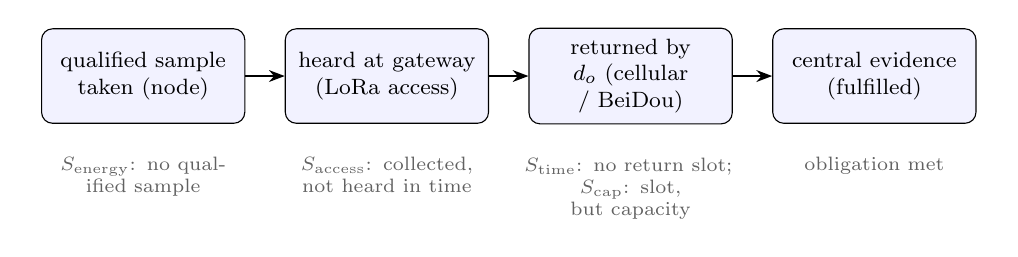
\begin{tikzpicture}[
  font=\footnotesize,
  box/.style={draw,rounded corners,align=center,inner sep=4pt,text width=23mm,
              minimum height=12mm,fill=blue!5},
  fail/.style={align=center,font=\scriptsize,text width=27mm,text=black!62},
  arr/.style={-{Stealth[length=2mm]},thick},
]
  \node[box] (s) {qualified sample taken (node)};
  \node[box,right=5mm of s] (h) {heard at gateway (LoRa access)};
  \node[box,right=5mm of h] (r) {returned by $d_o$ (cellular / BeiDou)};
  \node[box,right=5mm of r] (e) {central evidence (fulfilled)};
  \draw[arr] (s) -- (h);
  \draw[arr] (h) -- (r);
  \draw[arr] (r) -- (e);
  \node[fail,below=3mm of s] {$S_{\mathrm{energy}}$: no qualified sample};
  \node[fail,below=3mm of h] {$S_{\mathrm{access}}$: collected, not heard in time};
  \node[fail,below=3mm of r] {$S_{\mathrm{time}}$: no return slot;\newline $S_{\mathrm{cap}}$: slot, but capacity};
  \node[fail,below=3mm of e] {obligation met};
\end{tikzpicture}
\caption{The per-obligation chain and the four failure segments. An unfulfilled obligation is
charged to its \emph{first} failing stage under an optimistic model that grants every later
assumption, so the offline labels are mutually exclusive. An online observer that cannot see a
stage must return \emph{unknown} rather than guess it.}
\label{fig:chain}
\end{figure}

\paragraph{Energy and devices.}
A sample costs $4.7{\times}10^{-4}$~Wh;
an uplink costs $2.33{\times}10^{-5}$~Wh. Battery capacity is 0.05~Wh. Solar input follows a 12~h
half-sine with peak 0.03~Wh/h, with per-node/hour stochastic cloud occlusion. A node that browns
out \emph{permanently} dies in the main configuration (an absorbing state; a restart sensitivity
is left open). A cache of 240 slots with FIFO replacement sits at the node. Under the modelled
standard edge discipline a record leaves this cache only once it is acknowledged at the centre
(the acknowledgement is modelled synchronously and without airtime, a pre-existing simplification
that favours every queue discipline equally); until then it is retransmitted oldest-first, with at
most 32 records per upload opportunity. Access succeeds with probability 0.74; the primary
backhaul is good with probability 0.62.

\paragraph{Class~A execution reality.}
A configuration command is not immediate: it is queued, transits the backhaul to the gateway, and
reaches a node only in its next Class~A receive window; it counts as \textsc{applied} only when
the node later reports the new config. During a backhaul outage, commands are refused at admission
(they are never transmitted and occupy no airtime, so their count is a command-hygiene metric, not
a wireless or short-message billing saving). A command issued now, applied later, and still
consuming energy in between is a first-class effect; holding a dense 300~s regime across a 12~h
night needs $\approx$0.071~Wh, exceeding the 0.05~Wh battery.

\paragraph{Mission reachability and who knows what, when.}
The authorised schedule is piecewise (blue 600~s, then yellow 300~s from $t{=}6$~h). The centre is
pre-provisioned with the full authorised schedule; the \emph{field gateway's} obligation view,
however, is gated by a piecewise mission view and is published incrementally only as the mission
table traverses the backhaul. In the main scenario the primary is down from $t{=}4$~h to
$t{=}20$~h, and the table (which does not use the short-message path) reaches the gateway only at
$t{=}20$~h; before then the field lawfully continues the last \textsc{applied} blue configuration
under local autonomy. We therefore do not model the field learning of an unseen future task at
runtime; we model a pre-authorised schedule whose field view is delayed by the outage.

\paragraph{Three statement classes.}
Throughout, the runtime keeps distinct: \textbf{confirmed} (an independent node report shows the
target config, or a matching sample is received centrally); \textbf{unconfirmed} (a command is in
flight or receipts are incomplete---this implies neither that it took effect nor that the channel
is down); and \textbf{unreachable} (the current path is known down from an explicit network-side
state). A LoRa access receipt (``a node was heard'') is evidence about the access link only and can
never by itself establish backhaul reachability.

\paragraph{Strong baselines (the bar to beat).}
We assemble deliberately strong ordinary mechanisms with the same legal information:
\textbf{dayfeed}, an energy-aware policy that densifies by day and relaxes overnight;
\textbf{maxcov}, a max-coverage/recency greedy that packs each backup packet by marginal new
obligation coverage per byte; \textbf{piecewise mission views} with a gateway gate that withholds
future requirements until they arrive while preserving already-open windows; and \textbf{FIFO}
access repair. A scripted dayfeed decider driven through the full agent harness reproduces the
reference service level bit-for-bit, demonstrating no hidden privilege or penalty for the agent
path.

\section{The feasibility frontier, scoped to the policies tested}
\label{sec:frontier}

Before proposing any mechanism we ask whether controllable, changeable loss exists, using
\emph{symmetric} per-obligation counterfactuals: each relaxation widens one physical resource
(never the policy), and we report set differences over the same obligation ids, so a single
strategy's good luck cannot masquerade as an upper bound.

\paragraph{Failure-segment attribution (offline, time-aware).}
For every unfulfilled obligation we attribute the first blocking segment under an optimistic
model that favours feasibility: \stime when even the optimistic model finds no primary or backup
return opportunity between the qualified sample and $d_o$; \senergy when an opportunity exists but
no qualified sample is collected; \saccess when a sample is collected but is not heard at the
gateway \emph{by the deadline}; and \scap when it is heard in time but capacity/congestion cannot
return it. Only the first failing segment is charged. Over the full 48~h, of 7560 routine
obligations the strong maxcov/FIFO baseline delivers 3025 (0.400); the 4535 failures attribute
offline as \senergy\ 2002 (26.5\%), \scap\ 1945 (25.7\%), \stime\ 588 (7.8\%), \saccess\ 0. This
full-horizon accounting is an offline diagnostic; the online-visible subset is quantified in
\S\ref{sec:cert} and is substantially smaller.

\paragraph{Relaxation walls over the tested policy family.}
Table~\ref{tab:walls} relaxes energy (battery 0.05$\to$0.50~Wh with always-dense sampling) and
backhaul (the 1200~s/78~B point to 60~s with unlimited bytes) independently and jointly.
\begin{table}[h]
\centering\small
\resizebox{\linewidth}{!}{%
\begin{tabular}{llcc}
\toprule
Run & Sampling/Energy & Backhaul & Delivered \\
\midrule
base & dayfeed, 0.05~Wh & 1200~s/78~B & 3025 (0.400)\\
$O_{bh}$ & dayfeed, 0.05~Wh & unlimited & 4740 (0.627)\\
$O_{en}$ & always-300, 0.50~Wh & 1200~s/78~B & 4089 (0.541)\\
$O_{bo}$ & always-300, 0.50~Wh & unlimited & 6023 (0.797)\\
\bottomrule
\end{tabular}}
\caption{Counterfactual interventions over 7560 obligations. Set decomposition over the tested
configurations: 1715 obligations are blocked by backhaul capacity alone, 1128 by battery alone,
and 155 (2.0\%) require both. These are intervention results on the implemented strategies, not an
exhaustive optimum over all legal policies; we make no zero-remainder or global-optimality claim.}
\label{tab:walls}
\end{table}
These relaxations change resources \emph{and} couple in a specific policy, and the four-segment
labelling is an exhaustive partition of the implemented model rather than a proof that every
residual is physically immutable; we therefore read Table~\ref{tab:walls} as evidence that, for
the policy families we tested, the large fixed-resource gains require adding backhaul capacity or
energy, not smarter collection/scheduling/packing. A later section identifies one fixed-resource
gain that is orthogonal to all of these---a change to record \emph{lifetime disposition}
(\S\ref{sec:purge}), which was held constant here.

\paragraph{The sampling/energy policy family offers no robust operating point.}
A feed-forward night-energy policy that ignores two costs kills 13 nodes (service 0.213): it omits
the Class~A command latency $L$ (the node keeps sampling densely while the relax command
propagates) and the dawn charging ramp $R$ (solar input is near zero at sunrise). Counting both
($L{=}3600$, $R{=}7200$~s) collapses the policy bit-for-bit to dayfeed. A rolling-horizon MPC that
integrates the true half-sine harvest gains 1.47 points on seed~0 but averages $-1.3$ points over
six seeds and introduces 21 new permanent deaths on seeds dayfeed survives; a robust sweep over
the cloud coefficient has no operating point that adds no deaths and is not worse on average.
Legal information does not reveal tomorrow's clouds, while dense sampling under random cloud plus
an absorbing brownout state has asymmetric cost. This bounds the specific MPC/threshold policies
tested; it is not a claim that no energy controller can help under any formulation.

\paragraph{The outage window: mission unreachability dominates.}
\label{sec:outage}
Of the 2338 yellow obligations whose deadlines fall inside the outage (release$\geq$6~h,
deadline$\leq$20~h), removing the energy wall gives zero gain (the yellow command cannot traverse
the outage, so the field keeps sampling at blue 600~s regardless of battery), while widening the
backhaul adds 918; 1218 remain unfulfilled even under both interventions (no-slot geometry plus
access loss). An omniscient compile-time EDF packing that assumes every obligation's sample is
present at window start claims 420 obligations fit the backup slots, yet only 9 are realised---the
offline packing was optimistic about \emph{supply}, which the unreachable mission table prevents.
Feasibility projection must take the field's legally knowable supply rhythm as input, not the
nominal mission table.

\section{Feasibility statements under partial observability}
\label{sec:cert}

The runtime emits obligation-level statements, kept rigorously distinct: \textbf{fulfilled}
(verified by an independent scorer), \textbf{unconfirmed / not currently guaranteed} (a knowledge
boundary), and \textbf{infeasible-under-stated-conditions} (an optimistic model must also fail; a
heuristic that merely did not finish may never claim impossibility). Crucially, ``not currently
guaranteed'' is never upgraded to ``unreachable'' without network-side evidence.

\paragraph{Two placement levels.}
At \textbf{compile time (centre),} when an authorised change is authored, the centre holds the
full obligation table, the network-side outage status (current state, not a forecast of its
duration), and public device/link parameters. At \textbf{arrival time (gateway),} when a possibly
delayed mission table arrives, the gateway has the richest \emph{local} state---samples it has
actually heard, its own forwarding log, and backup slots used---but, by construction, nothing that
has not yet reached it.

\paragraph{Conditional structural no-return certificate (\stime).}
Backup slots occur at $t\bmod 1200{=}0$; an upgraded obligation's delivery window is 600~s. An
obligation whose window contains no backup slot cannot be returned via backup even under optimistic
supply and unlimited node energy; this is a geometric fact, seed-invariant. The certificate is
\emph{conditional}: it establishes \stime only \textbf{if the primary is in fact unavailable
across that window}. Given the network-confirmed outage interval $[4\mathrm{h},20\mathrm{h}]$, the
test emits 602 no-slot certificates; 588 obligations truly end as \stime (100\% recall of the 588,
zero false positives), with 14 obligations at the recovery edge (20~h) that an optimistic primary
slot could still serve and that are therefore excluded as boundary cases rather than certified.
Lead time ranges 0.2--14~h with median 7.2~h, \emph{conditional on the network-side unavailable
interval being known}; geometry alone never asserts an outage. A capacity certificate is
deliberately not issued at compile time because it is impure under our tests (552 correct \scap,
571 actually \senergy, 193 false positives); capacity attribution is pushed to the gateway.

\paragraph{Arrival-time attribution: online partial, offline complete.}
When the delayed table arrives at $t_{a}{=}20$~h, 2136 yellow obligations are already past
deadline. We contrast two attributions (Table~\ref{tab:attribution}). The \emph{offline,
time-aware} diagnostic uses simulator-wide evidence---whether a sample was ever taken, when it was
heard, and when it was returned---and labels all 2136 correctly. The \emph{online gateway-local}
attribution uses only evidence the gateway legally holds at $t_a$ (samples heard or received by
$t_a$) and returns an explicit unknown whenever the failure stage is not separable.
\begin{table}[h]
\centering\small
\begin{tabular}{lcc}
\toprule
Segment & Offline time-aware truth & Online gateway-local at $t_a$\\
\midrule
\stime (no return slot; geometry) & 588 & 588\\
\scap (heard by deadline, not returned) & 327 & 327\\
\saccess (heard after deadline / late) & 650 & 223\\
\senergy (no qualified sample) & 571 & --- (merged into unknown)\\
\unk (not separable online) & --- & 998\\
\midrule
Total & 2136 & 2136\\
Labelled coverage & 100\% & 53.3\% (1138/2136)\\
Precision on labelled subset & 1.000 & 1.000\\
\bottomrule
\end{tabular}
\caption{Arrival-time attribution of the 2136 upgraded obligations already missed when their
table reaches the gateway. Geometry needs no sample and is visible online; a sample heard by the
deadline but not returned is provably \scap to the gateway; a sample heard in
$(\text{deadline},t_a]$ is provably late access. The remaining 998 (46.7\%) have no sample heard
by $t_a$: the gateway cannot separate ``never sampled'' (\senergy, 571 in truth) from ``sampled
but heard only after $t_a$'' (\saccess, 427 in truth), and must report unknown under the original
G5 constraint. The earlier ``100\% arrival attribution'' was the offline column; it also merged
650 late-access cases into a 977-strong \scap class (977${=}327{+}650$).}
\label{tab:attribution}
\end{table}
The online-labelled subset is exact (1138/1138) but partial: 427 matching samples are first heard
after $t_a$, and 650 after their deadline. The result sharpens the runtime's requirement: the
projector must expose \emph{unknown} as a first-class state, and local mechanisms must be able to
act without resolving it.

\section{The obligation runtime: local release and execution placement}
\label{sec:purge}

\paragraph{Why withholding expired sends alone is not free.}
During the outage, expired backup records are the obvious reading of wasted metered capacity. But
under the hold-until-acknowledged discipline, withholding a backup record also withholds its
acknowledgement; the record stays in the node cache and, as an oldest unacknowledged entry, fills
the limited access batches, so genuinely fresh samples are not heard until the primary recovers.
At the main point, gateway-only suppression (stop sending expired records, leave the node cache
untouched) saves backup bytes but costs 8 on-time obligations (202$\to$194) and 0.25 service
points: cost is moved from the backhaul to the access segment, not removed.

\paragraph{Deadline-aligned expiry.}
The execution-layer counterpart releases an unacknowledged edge record when its business delivery
deadline has passed under the locally known period ($d\le t$)---a zero-false-positive test because
the deadline is absolute---while retaining every record with $d>t$. This both stops the expired
backup send and frees the access batch. We implement and compare two formulations. The node-local
\texttt{deadline-purge} needs no downlink at all; a gateway \texttt{cert-purge} locally
acknowledges records it will not send. We further implement \texttt{generic-expiry}, an ordinary
per-record expiration primitive: at record creation the source assigns a creation-relative
lifetime ending at the business deadline,
$\text{expires}=(\lfloor t_{\text{taken}}/P\rfloor+2)P$, expired records are deleted and their
retention released, unexpired records are kept, and survivors are sent FIFO. It references no
obligation id, return-slot geometry, or certificate.

\paragraph{The ``certificate'' mechanism is standard expiry.}
Across all ten seeds, \texttt{deadline-purge} and \texttt{generic-expiry} produce bit-identical
trajectories---identical service, outage on-time count, deaths, backup on-time/expired counts, and
the same delivered-obligation set (Table~\ref{tab:purgeexpiry}). We therefore make no
novel-discard-algorithm claim. Dropping stale or expired packets is well established in AoI packet
management and in DTN bundle expiry~\cite{costa2014pm,dtnarch,rfc9171}; BPv7 attaches a per-bundle
creation-time lifetime and deletes on expiry~\cite{rfc9171}. The system contribution is the
\emph{combination}: (i)~the lifetime is set from the obligation's end-to-end business delivery
deadline rather than packet age, a hop-local TTL, or an estimated single-packet delay; (ii)~release
is executed at the source with zero downlink, on evidence the source holds unconditionally; and
(iii)~disposition is consistent across the access and backhaul segments, which the
gateway-suppression experiment shows is necessary. Under a single fixed-period mission the
obligation-keyed and deadline-keyed formulations coincide; when one record supports several
overlapping obligations or mission versions, release must instead key to the \emph{latest} deadline
for which the record is still valid---a generalisation we leave to future work rather than claim.

\begin{table}[h]
\centering\small
\resizebox{\linewidth}{!}{%
\begin{tabular}{lcccc}
\toprule
Edge queue / action & Full svc (mean) & Outage on-time (10-seed total) & Expired backup records & Deaths\\
\midrule
maxcov + FIFO (baseline) & 0.373 & 1691 & 2538 & 12\\
maxcov + latest-only (AoI) & 0.358 & 4250 & 0 & 0\\
maxcov + \texttt{generic-expiry} (standard) & 0.415 & 4265 & 1 & 0\\
maxcov + \texttt{deadline-purge} (node) & 0.415 & 4265 & 1 & 0\\
\bottomrule
\end{tabular}}
\caption{Ten-seed sweep with the strong maxcov backup chooser fixed; only the edge disposition
changes. The standard per-record expiration and the prior ``certificate purge'' are bit-identical
on every seed. Expiry doubles outage on-time delivery while latest-only reaches outage freshness
by abandoning post-recovery coverage (lower full service). FIFO retains expired records and incurs
12 deaths. The gateway-only suppression point (not shown; same FIFO edge cache) gives 194 outage
on-time at seed~0 vs.\ 202 for FIFO and 434 for source expiry---the cross-segment cost.}
\label{tab:purgeexpiry}
\end{table}

\paragraph{Why ordinary reordering queues do not suffice.}
EDF and obligation-greedy disciplines reorder which records occupy a batch but never release
them, so the cache is not freed and we measure no gain. The AoI latest-only queue does release
records, but indiscriminately (it keeps only the newest), matching outage freshness while
permanently abandoning records still deliverable after recovery and lowering full-horizon
service. Deadline-aligned expiry supplies the \emph{selectivity} that turns a blunt freshness
heuristic into a service-preserving action; a fixed rule realises it, and an agent must maintain
the same deadline judgement when requirements change.

\paragraph{The local-certainty principle.}
The expiry result evidences the paper's central mechanism: at the moment $d\le t$ the node holds a
certain fact (its own record's business deadline has passed) whose required action (stop
retransmitting, free the batch) is entirely local, even though the node cannot know whether the
remote silence is a brownout, an access loss, or a backhaul outage. Complete chain diagnosis is
unnecessary for this disposition; demanding it would leave the worthless retransmission running.

\section{Execution locality and the layered runtime}
\label{sec:locality}

The source-expiry result hints at a placement principle; we make it explicit and test it
deterministically (no LLM, three seeds, the main operating point). A feasibility constraint can be
enforced in time at a layer only when three conditions jointly hold:
\[
\text{evidence available}\ \wedge\ \text{action authorised}\ \wedge\
D_{\text{observe}+\text{decide}+\text{act}} < M_c(t),
\]
where $M_c(t)$ is the remaining intervention window for constraint $c$. The question is not how
smart a centre planner is, but where these three hold.

\paragraph{Two deterministic mechanisms.}
The first is a centre-side feasibility \textbf{envelope}, a pure filter wrapping any planner
(rule, MPC, or LLM) and using only signals it may legally see (each node's last \emph{confirmed}
configuration, recent node-hearing counts, the authorised requirement, and the local clock). It
enforces a night-energy gate (18:00--06:00 sparse, dusk downgrade, 16:00--18:00 closed to new dense
sessions), a control-plane confirmation gate, and sparse-under-blue. The second is a
\textbf{node-local energy floor}: on every 60~s tick the node itself, on its local clock and
reported SoC, clamps sampling/report to sparse at night and self-downgrades at dusk with no centre
command; an optional pre-provisioned schedule additionally lets it execute the authorised
day/night rhythm locally. This models the ``pre-provisioned autonomous rules'' already in the
deployment; it is off by default and all pre-existing tests remain bit-identical when off. Unlike
the v4 advisory, the floor's night decision is a computed ledger (remaining dark hours $\times$
the dense-vs-sparse extra draw vs.\ reported SoC), not a blanket ``dense kills'' claim.

\paragraph{Why a centre envelope cannot ensure survival.}
A dense 300~s night costs $\approx$0.071~Wh, above the 0.05~Wh battery, and a brownout is absorbing
(permanent within the model). A centre-issued dusk downgrade must traverse the cellular backhaul
and then a Class~A receive window; under the outage and geometric loss it does not arrive before
dusk on the tightest-energy seed. The same rule---``never stay dense overnight''---is a late,
refusable \emph{suggestion} at the centre but an invariant enforced every tick \emph{at the node}.
Table~\ref{tab:r39} shows the consequence over the tested seeds.
\begin{table}[h]
\centering\small
\resizebox{\linewidth}{!}{%
\begin{tabular}{lcccc}
\toprule
Configuration (centre placement unless noted) & Mean svc & Deaths (3 seeds) & Cmds sent & Refused\\
\midrule
comply (na\"ive, no protection)                     & 0.162 & 39 & 160  & 2488\\
dayfeed-c (centre day/night rule)                   & 0.370 & 12 & 308  & 1256\\
envelope(comply), centre only                       & 0.359 & 12 & 308  & 298\\
comply + local floor                                & 0.366 & 0  & 1424 & 3364\\
dayfeed-c + local floor                             & 0.368 & 0  & 258  & 1156\\
\textbf{envelope(comply) + local floor}            & 0.359 & \textbf{0} & 282 & \textbf{222}\\
\midrule
local-dayfeed (existing conservative local policy) & 0.296 & 0  & 0    & 0\\
\textbf{pure-local (pre-provisioned, 0 centre cmd)} & \textbf{0.360} & \textbf{0} & 0 & 0\\
\bottomrule
\end{tabular}}
\caption{Deterministic three-seed placement study (no LLM). The local floor removes all permanent
deaths \emph{in the three tested seeds} at unchanged service; the envelope removes the command
storm (refused 2488$\to$222) but cannot save the tightest seed without the floor. Refused commands
are rejected at admission and never transmitted, so this is command hygiene, not a radio/short-
message billing saving. \emph{pure-local}---a node-local pre-provisioned rhythm with zero centre
commands---matches every centre-compiled service level for the tested static missions. The slightly
higher unprotected dayfeed-c mean is bought by 12 deaths and is not a survivable point. These are
point-specific empirical results, not a general survival guarantee or an optimal-controller bound.}
\label{tab:r39}
\end{table}

\paragraph{A local upper bound for static missions.}
\emph{pure-local} attains mean service 0.360 (range 0.317--0.387) with zero deaths and zero centre
commands, statistically indistinguishable from the centre-compiled configurations (0.359--0.368);
a run in which the centre still issues comply commands while the node executes the pre-provisioned
rhythm gives bit-identical service with 1274 sent / 2354 refused commands---centre sampling
commands are pure overhead under a static, predictable mission. This closes the centre
throughput/energy control question \emph{for the tested static, pre-provisioned missions}; it does
not bound non-pre-provisioned runtime task changes, which are the centre runtime's actual remit.

\paragraph{The layered runtime.}
The results prescribe three layers, each holding only constraints it can act on in time
(Figure~\ref{fig:layers}):
\textbf{L0, node-local (zero-signalling safety floor)}---the computed night-energy ledger and
deadline-aligned expiry, acting every tick on the node clock to prevent irreversible discharge and
dead-record cache exhaustion;
\textbf{L1, gateway-local (field autonomy)}---max-coverage backup packing, the non-prescient
mission-view gate, local (partial, unknown-aware) arrival attribution, and autonomous operation
during outages; and
\textbf{L2, centre agent runtime}---only what local autonomy cannot obtain: cross-layer
compilation and lawful re-compilation/renegotiation of \emph{non-pre-provisioned} authorised
changes, compile-time conditional structural certificates under the three-way statement
discipline, and honest external reporting. Every L2 action passes through the deterministic
envelope and can never override L0/L1. Rules, MPC, and solvers benefit from the same layers: this
is a general communication execution substrate, not a claim that an LLM is irreplaceable. Under
static pre-provisioned missions L2 rightly stays silent.

\begin{figure}[t]
\centering
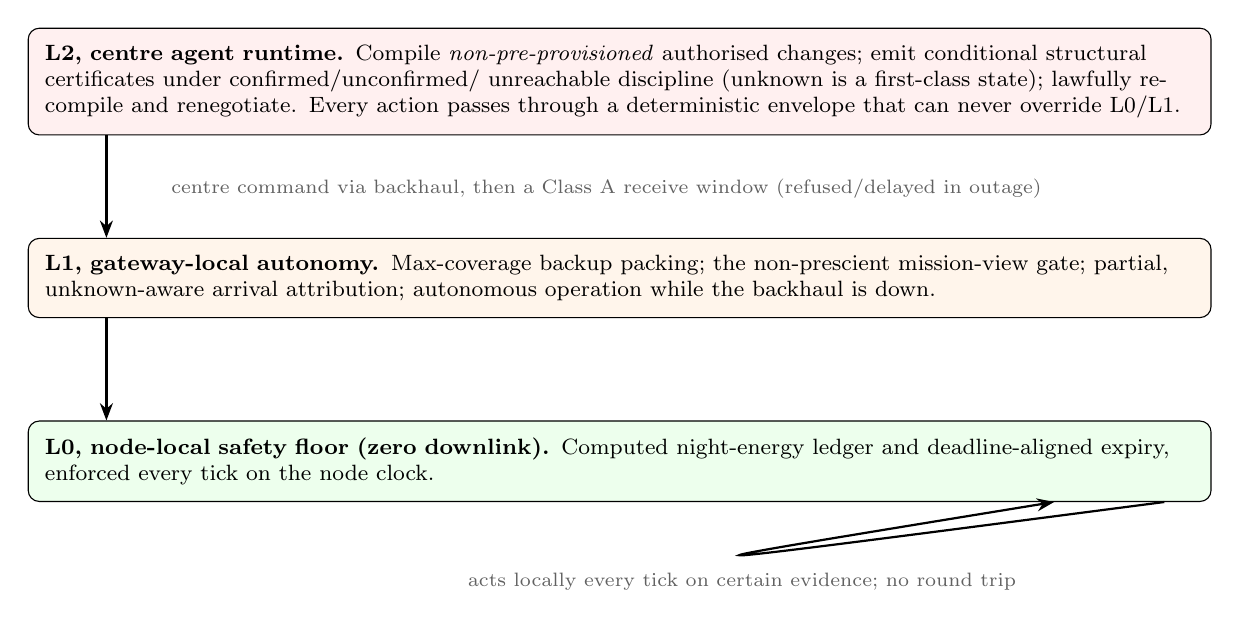
\begin{tikzpicture}[
  font=\footnotesize,
  layer/.style={draw,rounded corners,align=left,inner sep=6pt,text width=146mm},
  arr/.style={-{Stealth[length=2.2mm]},thick},
  note/.style={font=\scriptsize,align=left,text=black!62},
]
  \node[layer,fill=red!6] (L2){\textbf{L2, centre agent runtime.} Compile \emph{non-pre-provisioned}
    authorised changes; emit conditional structural certificates under confirmed/unconfirmed/
    unreachable discipline (unknown is a first-class state); lawfully re-compile and renegotiate.
    Every action passes through a deterministic envelope that can never override L0/L1.};
  \node[layer,fill=orange!8,below=13mm of L2] (L1){\textbf{L1, gateway-local autonomy.}
    Max-coverage backup packing; the non-prescient mission-view gate; partial, unknown-aware
    arrival attribution; autonomous operation while the backhaul is down.};
  \node[layer,fill=green!7,below=13mm of L1] (L0){\textbf{L0, node-local safety floor (zero downlink).}
    Computed night-energy ledger and deadline-aligned expiry, enforced every tick on the node clock.};
  \draw[arr] ($(L2.south west)+(10mm,0)$) -- ($(L1.north west)+(10mm,0)$);
  \node[note,anchor=west,text width=126mm] at ($(L2.south west)+(17mm,-6.8mm)$)
    {centre command via backhaul, then a Class~A receive window (refused/delayed in outage)};
  \draw[arr] ($(L1.south west)+(10mm,0)$) -- ($(L0.north west)+(10mm,0)$);
  \draw[arr] ($(L0.south east)+(-6mm,0)$) .. controls ($(L0.south)+(0,-9mm)$) ..
    ($(L0.south east)+(-20mm,0)$)
    node[midway,below=1mm,note]{acts locally every tick on certain evidence; no round trip};
\end{tikzpicture}
\caption{The layered obligation runtime. Safety-critical and deadline-certain constraints sit at
L0, where they act before energy or access opportunity is spent without any round trip; L1 holds
field-local packing and partial attribution; the L2 agent is confined to changes local autonomy
cannot obtain, and must report unconfirmed rather than unreachable without network-side evidence.}
\label{fig:layers}
\end{figure}

\section{Evaluation}
\label{sec:eval}

\textbf{Setup.} Seed~0 main point (with paired multi-seed checks where randomness enters): 48~h
plus a 1~h tail, 14 nodes in two groups, cap 0.05~Wh, solar peak 0.03~Wh/h, outage 4--20~h, backup
1200~s/78~B with maxcov, blue$\to$yellow (600$\to$300~s) at 6~h authorised at the centre with the
field mission table reaching the gateway at 20~h. Access $p{=}0.74$, primary backhaul
$p_{\mathrm{good}}{=}0.62$. All numbers are produced by repository scripts; each run reproduces the
repository checks and the five joint invariants; the local floor is off by default and the
disabled-backup/no-floor configurations remain bit-identical to the v1.1 anchors. The placement
study is deterministic over seeds 0--2; node death is a deterministic/highly robust quantity,
while mean-service differences below one point are not claimed significant. Seeds 6--9 are a
repeatedly reused held-out confirmation set, not an untouched test set.

\subsection{RQ1: Do structural certificates provide early, precise warning?}
\textbf{Conditionally, and deterministically.} Given the network-confirmed outage interval, the
geometry test emits 602 no-slot certificates; 588 obligations truly end as \stime (100\% recall,
zero false positives), the 14 recovery-edge cases are excluded rather than certified, and lead
time is 0.2--14~h (median 7.2~h). Without a confirmed unavailable interval the same geometry is
only a conditional statement (``unreturnable \emph{if} the primary stays down''), which is how we
now state it; geometry never infers an outage. An optimistic-energy capacity certificate is
impure (552 correct \scap, 571 actually \senergy, 193 false positives), so compile-time claims are
restricted to structural/unreachable segments and capacity attribution is pushed to the gateway.

\subsection{RQ2: What can the field attribute when the table finally arrives?}
\textbf{Partially online, completely offline (Table~\ref{tab:attribution}).} Using only evidence
held by $t_a{=}20$~h, the gateway labels 1138/2136 (53.3\%) missed upgraded obligations---all
geometric \stime (588), all in-time-but-not-returned \scap (327), and 223 provably late
\saccess---with 100\% precision on that labelled subset; 998 (46.7\%) are unknown, whose offline
truth is 571 never-sampled and 427 heard only after $t_a$. The offline time-aware diagnostic
labels all 2136 correctly (588/327/650/571); it also corrects the earlier online figure, which had
folded the 650 late-access cases into \scap. The runtime value at this level is therefore not
omniscient diagnosis but calibrated partial diagnosis plus an explicit unknown, which is exactly
the state the local mechanisms of \S\ref{sec:purge} operate despite.

\subsection{RQ3: Does deadline-aligned expiry recover wasted cost?}
During the outage 75 backup packets carry 750 records. With FIFO, of the records received
centrally via backup during the outage a large fraction arrive already expired (219 expired vs.\
261 on-time at seed~0, 45.6\%; 1270 of 2782 payload bytes). Gateway-only suppression removes those
sends but loses 8 on-time obligations (202$\to$194) through access back-pressure. Source-local
deadline expiry reverses the sign: at seed~0 it raises outage on-time obligations 202$\to$434 and
full-horizon service 0.400$\to$0.432, drives expired backup records to zero, and raises the
deadline-valid delivery fraction from 0.54 to 1.00; the gateway version is within 0.2 points
(0.430/420), confirming the gain is the deadline judgement rather than its location. Across ten
seeds (Table~\ref{tab:purgeexpiry}) expiry raises mean service 0.373$\to$0.415---a paired
$+4.21$ points (sd 0.81, 95\% CI $+3.64$ to $+4.79$, positive on all ten seeds)---and total
outage on-time delivery 1691$\to$4265 (2.52$\times$), with expired backup records 2538$\to$1 and
deaths 12$\to$0; it dominates AoI latest-only on every seed by $+5.73$ points (95\% CI $+5.06$ to
$+6.39$), because latest-only matches outage freshness only by abandoning post-recovery coverage.
EDF and obligation-greedy queues, which reorder but never release, gain nothing.

\subsection{RQ4: Does enforcement placement determine safety and command hygiene?}
\textbf{Yes, deterministically, within the tested seeds (Table~\ref{tab:r39}).}
(i)~Na\"ive centre compliance permanently kills 13/14 nodes on all three tested seeds (39 total)
and halves service to 0.162. (ii)~A centre envelope removes the command storm (refused
2488$\to$298) and protects two seeds but 12 nodes still die on the tightest seed because the dusk
downgrade cannot cross the backhaul and a Class~A window in time; the node-local floor removes all
39/12 deaths at unchanged service. (iii)~With the floor present, adding the envelope cuts refused
centre commands from 3364 (na\"ive) or 1156 (centre dayfeed) to 222 at the same zero-death service
level---a reduction in futile downlink \emph{attempts} (rejected at admission, not transmitted).
(iv)~A zero-command pre-provisioned rhythm reaches 0.360 service, matching every centre-compiled
arm for these static missions. We report zero deaths as an empirical result over the three tested
seeds and operating point, not a universal survival invariant, and we do not transcribe these
deterministic zeros onto the live agent runs of RQ5, which did not wire the L0 floor into the agent
loop.

\subsection{RQ5: What does a real agent show, and what does it not?}
\label{sec:agent}
We ran a live three-arm study with deepseek-flash over the 16~h outage (three seeds for an
unaided agent A0, the same agent with an ordinary pending-command checklist A0s, and a certificate
agent A1) plus two healthy-link controls, each a full 48~h$+$tail run with a real model call at
every 30~minute decision (99 decisions per trace). All arms share the harness, legal observation,
tools, history, and action space; only the decider's information block differs. We report the
service and death figures, then restate the honesty/accounting claims under symmetric scoring.

\paragraph{Service and survival (robust counts; noisy service at $n=3$).}
Table~\ref{tab:r38three} reports per-seed service and permanent deaths. A1 attains the highest
mean service (.358), statistically level with the deterministic safe floor (.360); seed-1 service
overlaps across arms, so we draw no service significance from $n=3$. Death counts are the more
robust quantity.
\begin{table}[h]
\centering\small
\resizebox{\linewidth}{!}{%
\begin{tabular}{lcccc}
\toprule
Arm & svc (s0/s1/s2) & svc mean & deaths (s0/s1/s2; total) & dense orders (3 outage seeds)\\
\midrule
A0 unaided & .160/.319/.408 & .296 & 13/13/9 (35) & 144\\
A0s + checklist & .181/.221/.265 & .222 & 13/13/13 (39) & 192\\
A1 + v4 certificate & .381/.316/.377 & .358 & 0/4/0 (4) & 67\\
\midrule
A0 healthy-link control & \multicolumn{2}{c}{.275} & 13 & 38\\
A1 healthy-link control & \multicolumn{2}{c}{.511} & 0 & 28\\
\bottomrule
\end{tabular}}
\caption{Live three-arm runs, 99 decisions per trace. The v0.6 ``false reports / infeasibility
log'' columns are removed: under symmetric relabelling they did not measure what they claimed
(see text). Dense orders count decisions that emitted a 300~s target. The four A1 seed-1 deaths
are \emph{not} cleared by L0 in this run, because the live agent loop was not wired to the L0
floor; the deterministic floor result of RQ4 is a separate experiment.}
\label{tab:r38three}
\end{table}

\paragraph{Accurate call accounting.}
The 11 traces contain 1089 decisions, not 1089 successful API calls. 52 decisions ended in a
parse-failure hold, caused by \texttt{max\_tokens} cutting the JSON mid-string (a second
thinking-disabled attempt then also failed); 412 decision records carry a first-attempt error even
when the retry succeeded (a logging artefact where the first error was not cleared). Per-arm
parse-failure rates are A0 7.1\% (28/396), A0s 6.4\% (19/297), A1 1.3\% (5/396): the arm
difference therefore mixes output-format reliability with any semantic effect of the certificate.
The hardened harness now logs per-request attempts, finish reasons, token use, and a truncation
marker for future runs.

\paragraph{The honesty claims must be restated.}
The v0.6 scorer (i)~scored a false ``upgrade in effect'' claim only inside decisions that ordered
dense, so an arm that mostly holds (A1) was scored on the empty set; (ii)~never ran on the
healthy-link group (its outage window was set to none), yielding initialisation zeros; and
(iii)~counted a broad keyword set (hold/guarantee/certificate/downgrade) that the certificate text
itself taught the model. Symmetric relabelling of every decision with denominators, plus the
interface fact that the observation's \texttt{link} field carries only LoRa access receipts
(\texttt{n\_heard}) and \emph{no backhaul state}, gives a different picture. In the forced outage
window, A0/A0s assert ``link up / commands can apply'' on 36/32 decisions (A1 on 2)---a
deterministic over-optimistic error, since the primary is down throughout; these are access
receipts misread as a live backhaul, and they accompany the ineffective dense orders and deaths.
Conversely, the v4 certificate asserts ``control plane not delivering'' whenever
$\text{heard}<n$; offline replay on the healthy-link control confirms five decision times
(local clock 14:00, 17:30 on day~1 and 07:00, 11:00, 06:30 on day~2) at which the primary was
usable yet the assertion fired---twice while 13/14 nodes had already confirmed the 300~s
regime---an over-pessimistic upgrade of \emph{unconfirmed} to \emph{unreachable}. The prior ``89 structural
infeasibility entries'' are prompt-taught wording (the corresponding terms appear in 317 A1
decisions and in zero A0/A0s decisions), not per-obligation structural registrations. The
honest finding is therefore not ``the certificate makes the model truthful'' but ``a missing
backhaul-state signal causes bidirectional errors, and the prompt packet changes both behaviour and
wording''; isolating the certificate's independent increment requires the matched-capability
control below.

\paragraph{Unknown-aware v5 projector (offline mechanism witness).}
We repaired the projector without re-running the LLM: unreachable is emitted only from an explicit
network-side current state (an observation field the current harness does not yet provide, in
which case the projector emits unconfirmed), and the night gate becomes a computed ledger
(remaining dark hours $\times$ the dense-vs-sparse extra draw vs.\ reported SoC) that distinguishes
ENERGY-INFEASIBLE from mere conservative advice. Replaying v4 and v5 over the same logged
observations: v5 issues zero unreachable assertions without a network-side field (v4 fired at all
five healthy-link false-alarm times; v5 labels them unconfirmed), and of the 528 dark decisions on
which v4 printed a blanket ``permanently kills'' gate, the ledger classifies 189 as genuinely
energy-infeasible and 339 as advisory---including every near-dawn decision (04:30--06:00), where
the remaining dense extra draw is small and reported SoC suffices. This is a counterfactual
mechanism witness, not an end-to-end v5 result.

\paragraph{Scope of the agent evidence.}
The live study is formative and single-model: it demonstrates the failure mode (access receipts as
backhaul state), the direction of the v4 packet's effect (fewer ineffective dense orders, fewer
deaths, but confounded with format reliability and expert heuristics), and the need for the v5
statement discipline. It does not establish an independent certificate increment (the A1 packet
also bundled day/night heuristics, geometric constants, confirmation rules, and note templates),
does not wire L0 into the agent, and is not a powered service-significance test. The deterministic
service, expiry, and safety results of RQ3/RQ4 do not depend on the LLM. The specified next
validation---a matched-capability arm that receives the same constants and heuristics without the
segment projector, v5 end-to-end runs with an explicit backhaul-state observation, and cross-model
replication---is left as future work.

\section{Related work}
\label{sec:related}
\textbf{LLMs in emergency / network control.} TopoLLM~\cite{topollm} uses an LLM with adaptive
tool learning for post-disaster emergency network topology planning; subsequent lines let LLMs
directly schedule UAV path/data collection and bandwidth, shape rewards for deep RL, or orchestrate
infrastructure-recovery tools, including graph-guided candidate-plan repair and LLM-driven operation
of real network-management APIs~\cite{icgrestore,ossgpt}. These decide \emph{network resources} or
compose recovery tools; intent objects, budget/time constraints, candidate-plan checks, and local
repair already appear in restoration systems, and LLM systems already orchestrate documented
APIs~\cite{icgrestore,ossgpt}, so we do not claim ``natural language to constraints'' as novel.
They do not maintain a long-horizon routine monitoring workflow across collection, configuration,
return, and recovery under intermittent links and tight energy, and do not maintain an
unknown-aware, three-class obligation state. Our delta is the per-obligation chain projection with
an explicit unknown, the conditional structural statement, and the local-certainty release
principle.

\textbf{Scheduling, freshness, energy.} An LLM in-context data-collection scheduler for
UAV-assisted sensor networks supplies the closest state-model precedent---per-sensor bounded
queues, exogenous arrivals, selectable objects under finite per-step service, battery/channel
state, and a verifier feedback loop~\cite{icldc}; AoI and energy-harvesting link optimisation,
including instantaneous-battery threshold policies and partially-observed energy-harvesting
control~\cite{bacinoglu1905,zakeri2311}, and overbooking/scheduled-aware forwarding for space
links~\cite{ccsdssabr} address pieces of the resource problem. Joint sampling/transmission/energy
optimisation is well established and we do not claim it; our distinction is remote
\emph{persistent} configuration with Class~A apply latency, the separated access vs.\
primary/backup return process, and---decisively---what the controller should \emph{say and lawfully
do} under partial observability when the mission is unfulfillable. Consistent network update work
has long studied per-update validity, dependencies, and loop-freedom during
transitions~\cite{sdnconsistency}; we rely on that lesson (versioning, dependencies, local repair
are not new). Network calculus and DTN triage under extreme contacts are complementary
deterministic characterisations of the walls we measure~\cite{leboudec01}.

\textbf{Packet discard, freshness, and DTN expiry.} Discarding stale or expired packets is well
established: AoI packet management pre-empts or drops old updates~\cite{costa2014pm,kam2016deadline,krishnan2019multihop};
deadline-aware buffer discard has been coupled with adaptive ARQ for video~\cite{razavivideo}; a
sensor transport suppresses generation when estimated delay exceeds a limit~\cite{wada2009timeout};
DTN bundle protocols attach a creation-time lifetime and expire bundles, alongside TTL/
encounter-based drop policies~\cite{dtnarch,iranmaneshdtnqueue,rfc9171}; LoRa--LEO rural IoT
systems instead schedule around estimated satellite contacts~\cite{sateriot}. Our source-local
disposition \emph{is} standard per-record expiration and we prove the equivalence; we claim not
the act of dropping but (i)~setting the lifetime from the obligation's end-to-end business
deadline rather than packet age, a local buffer deadline, an estimated single-packet delay, or a
bundle TTL; (ii)~requiring disposition to be consistent across the access and backhaul segments,
because withholding an expired backhaul send while the acknowledgement-driven FIFO repair cache
keeps the record back-pressures fresh access---a cross-segment interaction absent from single-hop
AoI discard and hop-local bundle expiry; and (iii)~retaining every still-rescuable record, which
AoI latest-only (whose objective ignores coverage) does not. DTN custody transfer~\cite{rfc5050}
moves retention responsibility as a \emph{forward} hand-off to decouple reliability from any
end-to-end acknowledgement, keyed to custody rather than an obligation deadline, and has been
migrated out of the BPv7 core~\cite{rfc9171}; it is an alternative architecture for the
responsibility transfer we measure at the source, and a deployment study of custody hand-off
versus source expiry is complementary future work.

\section{Discussion, limitations, and threats to validity}
\label{sec:disc}
\textbf{Scope of claims.} The throughput negative result is established at one main operating
point against symmetric relaxations and strong (omniscient, MPC, greedy) baselines, and is scoped
to the policy families tested; we make no global optimality or zero-remainder claim, and a better
formulated controller could exist. The conditional \stime certificate is geometric and
seed-invariant but presupposes a network-side unavailable interval; without it the statement is
only conditional. Online arrival attribution is deliberately partial (53.3\%, exact on the
labelled subset); treating its unknowns as a known segment would recreate the exact error we
correct, and a deployment that can supply current (not forecast) backhaul state to the centre can
shrink the unknown class---the v5 projector already consumes such a field.

\textbf{Agent evidence.} The live study uses one model with three outage seeds per arm (plus two
healthy controls), each a single temperature-0 trajectory; per-run service variance is large at
$n=3$, and the arm contrast confounds the segment projector with expert heuristics, geometric
constants, note templates, and output-format reliability (parse-failure rates differ 5-fold). The
hardened harness (per-request accounting, symmetric scoring over every decision and both groups,
the v5 unknown-aware projector and energy ledger) is in the repository so that the specified
matched-capability, v5 end-to-end, and cross-model studies can be run without re-litigating the
instrumentation; those runs are explicitly not claimed here. The live agent loop was not wired to
the L0 floor, so deterministic RQ4 zeros are not transcribed to agent deaths.

\textbf{Expiry assumptions.} The central acknowledgement is modelled synchronously and without
airtime, a pre-existing simplification that favours every queue discipline; the source-local
expiry needs no downlink and is our primary mechanism, while gateway acknowledgements would consume
Class~A receive windows in deployment. During the outage the node tests deadlines against the
public pre-change period $P{=}600$; the post-upgrade $P{=}300$ deadline enters only post-hoc
accounting, never as an online input. The equivalence of obligation-keyed and deadline-keyed
release holds for a single fixed-period mission; multi-obligation or mission-version overlap,
where one record remains valid for a later obligation, requires release keyed to the record's
latest still-valid deadline and is left future work, as is a custody-transfer deployment
comparison. Expired records forgo retrospective value after their deadline; where that matters
they can be retained at the gateway rather than sent.

\textbf{Model and provenance.} The brownout model is absorbing; a restart sensitivity could move
the energy wall but not the slot/capacity walls. Wider deployment ranges (backup rate/payload,
node count, capacity, cloud cover, restart threshold) are not swept, and sub-point mean-service
differences are not treated as significant. Centre knowledge of the outage interval assumes
network-side operations visibility of the \emph{current} state, not its duration; a conservative
variant counts only deterministic backup slots. Standards text for one channel was obtained from
a document-sharing host (top-grade document, lower-grade copy chain) because the official host was
unreachable by TLS from our environment; clause numbers were cross-checked from two independent
copies, and the international LoRa-plus-satellite and some vendor lines were not verified and are
not used as fact. We did not execute cited systems' reference implementations and claim no
replication of them; one field-study endpoint was rate-limited from our network and is cited
without its numbers.

\textbf{Generality.} The obligation chain, the three-class statement discipline with an explicit
unknown, and the local-certainty release principle transfer to any intermittent, energy-limited,
authority-bounded monitoring workflow; the specific walls and periods are parameterised by the
deployment and must be re-derived per deployment.

\section{Conclusion}
For pre-disaster geohazard monitoring under intermittent connectivity, strong ordinary
controllers already extract essentially all the on-time delivery that fixed resources allow over
the policies we tested; the failures that remain are physical and, offline, cleanly attributable.
The defensible role of an agent runtime is therefore neither to out-pack the network nor to drive
safety-critical sampling, but to sit above a layered, execution-grounded obligation runtime. We
separate what the field can know from what it cannot: at gateway arrival less than half of missed
upgraded obligations admit an exact segment label from local evidence and the rest must remain
unknown, while complete attribution is an offline capability. That partial observability does not
paralyse the edge---a node holds certain knowledge of its own records' business deadlines and can
stop worthless retransmission and night-time discharge without diagnosing the remote cause. This
deadline-aligned expiry is a standard primitive whose value lies in its business-deadline basis,
its zero-downlink source placement, and its cross-segment consistency, doubling outage on-time
delivery while removing expired sends and deaths where gateway-only suppression merely moves cost
to the access segment. Safety-critical constraints sit at the node because only there the
observe-decide-act delay beats the intervention window; the centre is confined to
non-pre-provisioned authorised changes and to statements that never upgrade unconfirmed to
unreachable. A formative real-agent study confirms the interface failure this design targets and
motivates the unknown-aware projector, while the deterministic guarantees rest on rules any
planner can use. The result is a runtime that promises only what it can execute, says unknown when
it cannot tell, and still acts---locally and correctly---on the things it knows for certain.

\bibliographystyle{unsrt}
\bibliography{refs}

\end{document}
